\section{Механизмы обеспечения конфиденциальности в СУБД}
\subsection{Классификация угроз конфиденциальности СУБД}

\subsubsection{Причины, виды, основные методы нарушения конфиденциальности}

Конфиденциальность – состояние информации, при котором доступ к ней осуществляют только субъекты,
имеющие на него право.

Основными причинами нарушения конфиденциальности информации являются \cite{o-salo}:
\begin{itemize}
    \item несоблюдение персоналом норм, требований, правил эксплуатации АС
    \item ошибки в проектировании АС и систем защиты АС
    \item ведение противостоящей стороной технической и агентурной разведок
\end{itemize}

Угрозы конфиденциальности информации направлены на несанкционированное перемещение информации от
носителя-источника к носителю-получателю (угроза разглашения, утечки, несанкционированного доступа).
Уязвимость информации к преднамеренным действиям злоумышленников или иных заинтересованных лиц является
наиболее опасной. Как уже отмечалось выше, различные виды уязвимости обусловлены угрозами разглашения, НСД %%утечки информации.
Уязвимость информации к разглашению – несанкционированному сообщению защищаемой информации лицам, не меющим
%права доступа к ней, – определяется, прежде всего, неправильной организацией работы с информацией и е
%носителями, а также неосторожными или умышленными действиями людей, допущенных к работе с данной информацией.

Уязвимость информации к НСД – противоправному преднамеренному овладению защищаемой информацией лицом,
не имеющим права доступа к ней, – определяется наличием у информации, ее носителя или у самой системы
защиты недостатков, которые создают возможность получения информации, ее модификации, уничтожения,
блокирования доступа к ней.

Уязвимость информации к утечке – неконтролируемому распространению защищаемой информации за пределы круга лиц,
которым эта информация была доверена, – возникает, как и в случае разглашения, из-за неправильной организации
работы с информацией, а также в связи с "дырами" в системе защиты информации, неосторожными или умышленными
действиями людей, допущенных к работе с защищаемыми сведениями. Утечка может происходить по акустическому,
визуально-оптическому, материально-вещественному и электромагнитному каналам. Следовательно, уязвимость
информации к утечке определяется слабыми сторонами носителя информации, среды, окружающей информацию,
и технических средств, находящихся в непосредственной близости от носителей информации \cite{univermvd-eios}.


Также, угрозы делят на умышленные и неумышленные(баги в ПО, сгнили провода и тп), умышленные в свою
очередь делят на активные и пассивные:
\begin{itemize}
    \item Активные угрозы имеют целью нарушение нормального функционирования ИТ посредством
        целенаправленного воздействия на аппаратные, программные и информационные ресурсы.
    \item Раскрытие конфиденциальной информации - это бесконтрольный выход конфиденциальной
        информации за пределы информационной технологии или круга лиц, которым она была доверена по
        службе или стала известна в процессе работы.
\end{itemize}

Умышленные угрозы подразделяются также на следующие виды:
\begin{itemize}
    \item Внутренние - возникают внутри управляемой организации. Они чаще всего сопровождаются
        социальной напряженностью и тяжелым моральным климатом на экономическом объекте, который
        провоцирует специалистов выполнять какие-либо правонарушения по отношению к информационным ресурсам
    \item Внешние - Пассивные угрозы направлены на несанкционированное использование информационный
        ресурсов, не оказывая при этом влияния на функционирование ИТ
\end{itemize}

Далее приведены некоторые угрозы ИБ.

\textbf{Раскрытие конфиденциальной информации} - это бесконтрольный выход конфиденциальной
информации за пределы информационной технологии или круга лиц, которым она была доверена по
службе или стала известна в процессе работы.

Раскрытие конфиденциальной информации может быть следствием:
\begin{itemize}
    \item разглашения конфиденциальной информации
    \item утечки информации по различным, главным образом техническим, каналам
        (по визуально-оптическим, акустическим, электромагнитным и др
    \item несанкционированного доступа к конфиденциальной информации различными способами
\end{itemize}

\textbf{Несанкционированный доступ к информации} выражается в противоправном преднамеренном
овладении конфиденциальной информацией лицом, не имеющим права доступа к охраняемым сведениям.

Наиболее распространенными путями несанкционированного доступа к информации являются:
\begin{itemize}
    \item перехват электронных излучений
    \item принудительное электромагнитное облучение (подсветка) линий связи с целью получения
        паразитной модуляции несущей
    \item применение подслушивающих устройств (закладок)
    \item дистанционное фотографирование
    \item перехват акустических излучений и восстановление текста принтера
    \item чтение остаточной информации в памяти системы после выполнения санкционированных запросов
    \item копирование носителей информации с преодолением мер защиты
    \item маскировка под зарегистрированного пользователя ("маскарад")
    \item использование недостатков языков программирования и операционных систем
\end{itemize}

Перечисленные пути несанкционированного доступа требуют достаточно больших технических знаний и
соответствующих аппаратных или программных разработок со стороны взломщика. Например, используются
технические каналы утечки - это физические пути от источника конфиденциальной информации к
злоумышленнику, посредством которых возможно получение охраняемых сведений. Причиной возникновения
каналов утечки являются конструктивные и технологические несовершенства схемных решений либо
эксплуатационный износ элементов. Все это позволяет взломщикам создавать действующие на определенных
физических принципах преобразователи, образующие присущий этим принципам канал передачи информации
- канал несанкционированного доступа.

\textbf{Несанкционированное использование информационных ресурсов}, с одной стороны, является
последствиями ее утечки и средством ее компрометации. С другой стороны, оно имеет самостоятельное
значение, так как может нанести большой ущерб управляемой системе (вплоть до полного выхода
информационной технологии из строя) или ее абонентам.

\textbf{Незаконное использование привилегий.} Любая защищенная технология содержит
средства, используемые в чрезвычайных ситуациях, или средства, которые способны
функционировать с нарушением существующей политики безопасности. Например, на случай
внезапной проверки пользователь должен иметь возможность доступа ко всем наборам
системы. Обычно эти средства используются администраторами, операторами, системными
программистами и другими пользователями, выполняющими специальные функции.
Большинство систем защиты в таких случаях используют наборы привилегий, т. е. для
выполнения определенной функции требуется определенная привилегия. Обычно
пользователи имеют минимальный набор привилегий, администраторы - максимальный.
Наборы привилегий охраняются системой защиты. Несанкционированный (незаконный)
захват привилегий возможен при наличии ошибок в системе защиты, но чаще всего
происходит в процессе управления системой защиты, в частности, при небрежном
пользовании привилегиями.

\textbf{"Взлом системы"} - умышленное проникновение в информационную технологию, когда взломщик не
имеет санкционированных параметров для входа. Способы взлома могут быть различными, и при некоторых
из них происходит совпадение с ранее описанными угрозами. Например, использование пароля пользователя
информационной технологии, который может быть вскрыт, например, путем перебора возможных паролей \cite{system-hack}.


\subsubsection{Типы утечки конфиденциальной информации из СУБД, частичное разглашение}

Утечки информации — неправомерная передача конфиденциальных сведений (материалов, важных для различных
компаний или государства, персональных данных граждан), которая может быть умышленной или случайной.
Утечка информации возможна по разным причинам.

Умышленные утечки:
\begin{itemize}
    \item Инсайдеры и избыточные права. К этому виду относятся случаи, основной причиной которых
        стали действия сотрудников, имеющих доступ к секретам легально, в силу своих служебных
        обязанностей. Все варианты инсайда условно можно разделить на две группы: в одном случае
        сотрудник, не имея доступа к информации, получает ее незаконно, а в другом он обладает
        официальным доступом к закрытым данным и умышленно выносит их за пределы компании.
    \item Кража информации (извне). Проникновение в компьютер с помощью вредоносных программ и
        похищение информации с целью использования в корыстных интересах. На хакерские атаки
        приходится 15\% от всего объема утечек информации. Вторжение в устройство извне и
        незаметная установка вредоносных программ позволяют хакерам полностью контролировать
        систему и получать доступ к закрытым сведениям, вплоть до паролей к банковским счетам и
        картам. Для этого могут применяться различные программы вроде «троянских коней». Главный
        атрибут данного вида утечки — активные действия внешних лиц с целью доступа к информации.
    \item Взлом программного обеспечения. Приложения, используемые в рабочем процессе или на личном
        компьютере сотрудника, часто имеют незакрытые уязвимости, которые можно эксплуатировать и
        получать тем самым различные небезопасные возможности вроде исполнения произвольного кода или
        повышения привилегий.
    \item Вредоносные программы (бекдоры, трояны) нацелены на причинение вреда владельцу устройства,
        позволяют незаметно проникать в систему и затем искажать или полностью удалять информацию,
        подменять ее другими,  похожими данными.
    \item Кражи носителей. Весьма распространенный вариант утечек, который случается в результате
        преднамеренного хищения устройств с информацией — ноутбуков, смартфонов, планшетов и других
        съемных носителей данных в виде флешек, жестких дисков.
\end{itemize}

Случайные утечки. К этому виду можно отнести инциденты, которые происходят из-за потери носителей
данных (флешек, ноутбуков, смартфонов) или ошибочных действий сотрудников организации. Результатом
может быть размещение конфиденциальной информации в интернете. Также не последнюю роль играет
человеческий фактор, когда сотрудник по недосмотру открывает доступ к закрытым данным всем желающим \cite{leaks}.


\subsubsection{Соотношение защищенности и доступности данных}
Поддержание слишком жесткой политики безопасности может негативно
сказаться на надежности функционирования опреционной системы.

Если например, в Windows запретить псевдопользователю SYSTEM, от имени которого выполняются
системные процессы, доступ к исполняемым файлами системныъ процессов, операционная система не
сможет загрузиться. В данном случае чрезмерно жесткая политика безопасности приводит к
моментальному краху операционной системы, в других случаях подобная политика безопасности может
приводить к трудновыявляемым ошибкам и сбоям в процессе функционирования операционной системы,
что ещё более опасно.

Таким образом, при определении адекватной политики безопасности не следует пытаться достигнуть
максимально возможного уровня защищённости операционной системы. Оптимальная адекватная политика
безопасности - такая политика безопасности, которая не только не позволяет нарушителям выполнить
несанкицонированные действия, но и не приводит к вышеописанным негативным последствия.

Не существует единой адекватной политики безопасности на все случаи жизни. То, какая политика
безопасности будет адекватной, определяется не только архитектурой операционной системы, но и её
конфигурацией, ассортиментом установленного программного обеспечения и т.д. Политика безопасности,
адекватная для некоторой операционной системы, скорее всего, будет неадекватна для другого
экземпляра той же операционной системы. Бользинство современных систем достаточно универсальны и
могут применяться для решения самых разных задач. Одна и та же операционная система может
использоваться для обеспечения функционирования автоматизированной бановской системы, веб-сервера,
системы электронного документооборота. Очевидно, что угрозы безопасности для всех трёх указанныъ
применений будут различны и адекватная политика безопасносит в каждом из трёх случаев будет своя.

Формирование и поддержание адекватной политики безопасности операционной системы в общем случае
можно разделить на следующие этапы \cite{os-protection}.
\begin{enumerate}
    \item \textbf{Анализ угроз.} Администратор операционной системы рассматривает возможные угрозы
        безопаснотсти данного экземпляра операционной системы. Среди возможных угроз выделяются
        наиболее опасные, защите от которых нужно уделять максимум сил и средств.
    \item \textbf{Формирование требований к политике безопасности.} На этом этапе администратор
        определяет, какие средства и методы будут применяться для защиты от тех или иных угроз.
        Например, защиты от несанкционированного доступа к некотторому объекту операционной системы
        можно решать либо средствами разграничения доступа, либо криптографическими средствами, либо
        используя некоторую комбинацию этих средств, либо используя какие-то иные средства. На данном
        этапе администратор должен сделать подоный выбор для каждой угрозы безопасности операционной
        системы, выбирая оптимальные средства защиты от каждой угрозы. Одновременно администратор
        анализирует возможные побочные эффекты различных вариантов политики безопасности, оцениваня,
        в какой мере в каждом варианте политики безопасносит буду проявляться побочные негативные
        факторы. Как правило, администратору приходится идти на компромисс, смиряясь либо с
        недостаточной защищённостью операционной системы от отдельных угроз, либо с определёнными
        трудностями пользователей при работе с ситемой. Результатом данного этапа является набор
        требований неподобие: "В операционной системе должно быть предусмотрено дискрециаонное
        разграничение доступа с минимизацией полномочий пользователей и частичной реализацией правил
        изолированной программной среды".
    \item \textbf{Формальное определение политики безопасности.} Данный этап заключается в том, что
        администратор четко опеределяет, как конкретно должны выполняться требования, сформулированные
        на предыдущем этапе. Администратор решает, можно ли добиваться выполнения этих требований
        только встроенными средствами операционной системы или необходима установка дополнительных
        пакетов защиты. В последнем случае производится выбор необъодимого программного обеспечения. На
        данном этапе формулируются необходимые требования к конфигурации операционной системы, а также
        требования к конфигурации дополнительных пакетов защиты, если установка таких пакетов
        необходима. Кроме того, на данном этапе администратор должен предусмотреть порядок внесения
        необходимых изменений в политику безопасности в чрезвычайных ситуациях, например, при
        обнаружении факта несанкционированного входа в систему пользователя-нарушителя. Результатом
        данного этапа является развернутый перечень настроек конфигурации операционной системы и
        дополнительных пакетов защиты с указанием того, в каких ситуациях какие настройки должны быть
        выставлены.
    \item \textbf{Претворение в жизнь политики безопасности.} К началу этого этапа у администратора
        операционной системы имеется чёткое представление о том, какой должна быть адекватная политика
        безопасности. Задачей этапа является приведение конфигурации операционной системы и
        дополнительных пакетов защиты в соответсвие с политикой безопасности, формально определённой
        на предыдущем этапе.
    \item \textbf{Поддержание и коррекция политики безопасонсти.} На данном этапе операционная
    система функционирует в соотвтествии с политикой безопасности, определённой на третьем этапе.
    Задачей администратора является конторль над соблюдением политики безопасности и внесение в неё
    необходимых изменений по мере появления изменений в функционировании операционной системы.
    Например, если в операционной системе устанавливается новый программный продукт, может
    потребоваться коррекция политики безопасности таким образом, чтобы этот программный продукт мог
    нормально функционировать.
\end{enumerate}


\subsubsection{Получение несанкционированного доступа к конфиденциальной информации путем логических выводов}
Нередко путем логического вывода можно извлечь из базы данных информацию, на получение которой
стандартными средствами у пользователя не хватает привилегий.

Если для реализации контроля доступа используются представления и эти представления допускают
модификацию,
%помощью операций модификации/вставки можно получить информацию о содержимом базовых таблиц, не располагая прямым доступом к ним.

Основным средством борьбы с подобными угрозами, помимо тщательно проектирования модели данных,
является механизм размножения строк. Суть его в том, что в состав первичного ключа, явно или неявно,
включается метка безопасности, за счет чего появляется возможность хранить в таблице несколько
экземпляров строк с одинаковыми значениями "содержательных" ключевых полей. Наиболее естественно
размножение строк реализуется  СУБД, поддерживающих метки безопасности (например, в INGRES/
Enhanced Security), однако и стандартными SQL-средствами можно получить удовлетворительное решение.

Рассмотрим базу данных, состоящую из одной таблицы с двумя столбцами - имя пациента и диагноз.
Предполагается, что имя является первичным ключом. Каждая из строк таблицы относится к одному
из двух уровней секретности - высокому (HIGH) и низкому (LOW). Соответственно, и пользователи
подразделяются на два уровня благонадежности, которые мы также будем называть высоким и низким.
К высокому уровню секретности относятся сведения о пациентах, находящихся под надзором
правоохранительных органов или страдающих специфическими заболеваниями. На низком уровне
располагаются данные о прочих пациентах, а также информация о некоторых "секретных" пациентах
с "маскировочным" диагнозом. Части таблицы могут выглядеть примерно так:

\begin{figure}[h]
    \centering
    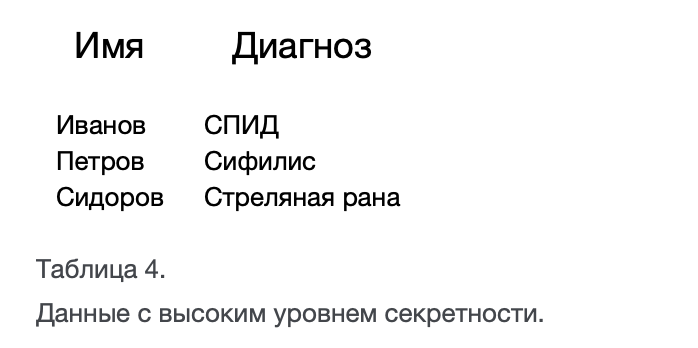
\includegraphics[width=0.8\textwidth]{assets/diagnoses1.png}
\end{figure}

\begin{figure}[h]
    \centering
    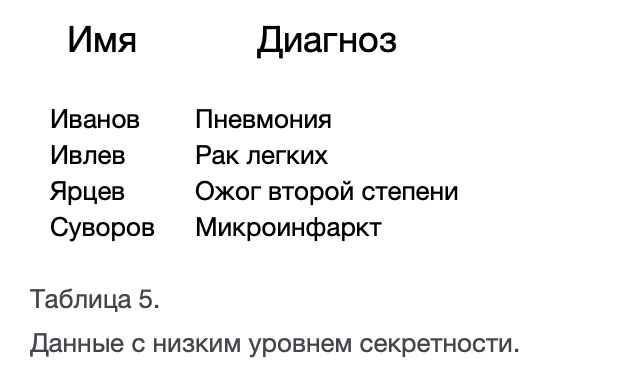
\includegraphics[width=0.8\textwidth]{assets/diagnoses2.png}
\end{figure}

Обратим внимание на то, что сведения о пациенте по фамилии Иванов присутствуют на обоих уровнях,
но cодержат разные диагнозы.

Мы хотим реализовать такую дисциплину доступа, чтобы пользователи с низким уровнем благонадежности
могли манипулировать только данными на своем уровне и не имели возможности сделать какие-либо
выводы о присутствии в секретной половине сведений о конкретных пациентах. Пользователи с высоким
уровнем благонадежности должны иметь доступ к секретной половине таблицы, а также к информации о
прочих пациентах. Дезинформирующих строк о секретных пациентах они видеть не должны:

\begin{figure}[h]
    \centering
    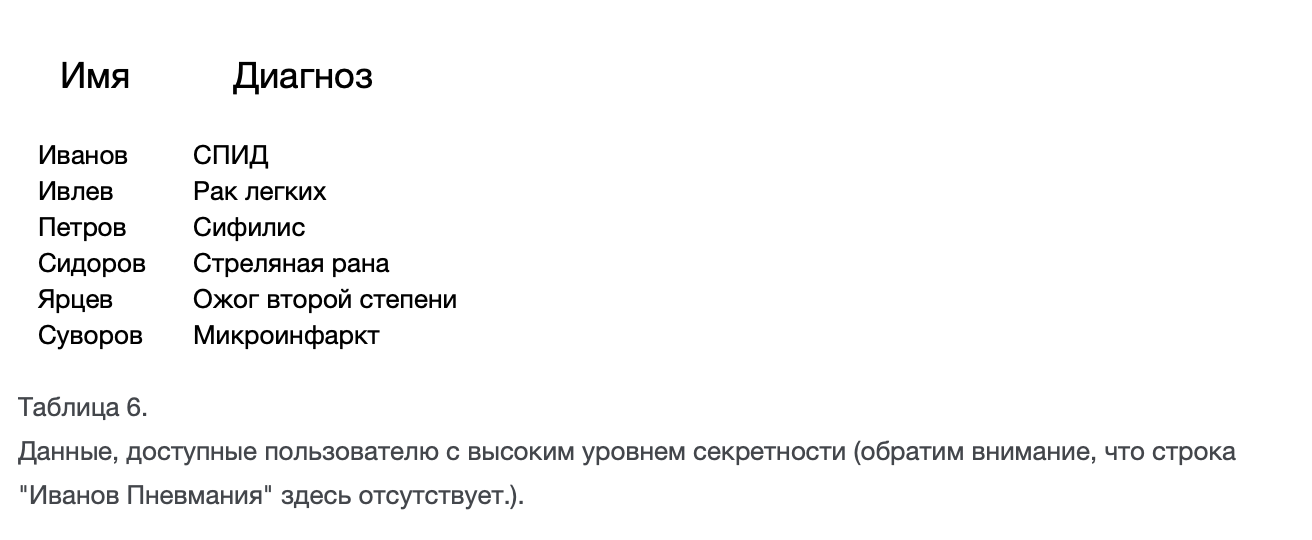
\includegraphics[width=0.8\textwidth]{assets/diagnoses3.png}
\end{figure}


\subsubsection{Методы противодействия. Особенности применения криптографических методов}

\paragraph{Криптосистемы.}

Для описания различных методов в криптографии используется понятие криптографической системы или
\textbf{криптосистемы}.
Криптографические системы и шифры можно разделить на две большие группы в зависимости от принципа
использования ключей для шифрования и расшифрования \cite{crypto-methods}:
\begin{itemize}
    \item \textbf{Симметричная криптосистема.} Для шифрования и расшифрования используется один и
        тот же ключ $\mathit{K}$, либо если получение ключа расшифрования $\mathit{K_2}$ из ключа
        шифрования $\mathit{K_1}$ является тривиальной операцией. В зависимости от объёма данных,
        обрабатываемых за одну операцию шифрования, симметричные шифры делятся на блочные, в
        которых за одну операцию шифрования происходит преобразование одного блока данных (32 бита,
        64, 128 или больше), и потоковые, в которых работают с каждым символом открытого текста по
        отдельности (например, с 1 битом или 1 байтом). Использование блочного шифра подразумевает
        разделение открытого текста на блоки одинаковой длины, к каждому из которых применяется
        функция шифрования. Кроме того, результат шифрования следующего блока может зависеть от
        предыдущего. В качестве примеров симметричных криптосистем можно привести международные
        стандарты DES и пришедший ему на смену AES, оба являются Блочными. Пример потокового - RC4,
        который также может выступать в качетве генератора псевдослучайной последовательности
        случайных чисел.
    \item \textbf{Ассимитричная криптосистема или криптосистема с открытым ключом.} Получить ключ
        расшифрования из ключа шифрования вычислительно сложно. Некоторые из них рассмотрены в
        главе 9. Все используемые на сегодняшний день асимметричные криптосистемы работают с
        открытым текстом, составляющим несколько сотен или тысяч бит, поэтому классификация таких
        систем по объёму обрабатываемых за одну операцию данных не производится. Алгоритм, который
        выполняет отображение аргумента произ- вольной длины в значение фиксированной длины,
        называется хэш-функцией. Если для такой хэш-функции выполняются определён- ные свойства,
        например, устойчивость к поиску коллизий, то это уже криптографическая хэш-функция.
        Для проверки аутентичности сообщения с использованием об- щего секретного ключа
        отправителем и получателем используется код аутентификации [сообщения] (другое название в
        русскоязыч- ной литературе - имитовставка, англ. message authentication code, MAC ),
        рассмотренный в разделе 8.3. Его аналогом в криптосисте- мах с открытым ключом является
        электронная подпись, алгорит- мы генерации и проверки которой рассмотрены в главе 9 вместе
        с алгоритмами асимметричного шифрования. Примеры асимметричных криптосистем – RSA и схема
        Эль-Гамаля.
\end{itemize}

Симметричные и асимметричные криптосистемы, а также различные их комбинации используются в АС
прежде всего для шифрования данных на различных носителях и для шифрования трафика.


\paragraph{Применение шифрования в базах данных.}

Шифрование базы данных — использование технологии шифрования для преобразования информации,
хранящейся в базе данных (БД), в шифротекст, что делает её прочтение невозможным для лиц, не
обладающих ключами шифрования.

Основные подходы можно классифицировать по тому, на каком уровне и на какой стороне происходит шифрование:
\begin{itemize}
    \item Шифрование на уровне хранилища.
    \item Шифрование на уровне базы данных.
    \item Шифрование на уровне приложения.
    \item Шифрование на стороне клиента. (Zero-knowledge database)
\end{itemize}

\subparagraph{Шифрование на уровне хранилища.}
Также называемое «прозрачным» (Transparent Database Encryption, TDE). Данная технология,
применяется, например, в продуктах Microsoft и Oracle для шифрования и дешифрования ввода-вывода
файлов БД. Данные шифруются перед записью на диск и дешифруются во время чтения в память, что
решает проблему защиты «неактивных» данных, но не обеспечивает сохранность информации при передаче
по каналам связи или во время использования. Преимуществом TDE является то, что шифрование и
дешифрование выполняются прозрачно для приложений, то есть их модификация не требуется.

Реализация шифрование на уровне хранилища Microsoft.

TDE применяется для файлов БД и журнала транзакций на уровне страниц. Страницы шифруются с помощью
специального симметричного ключа шифрования базы данных (англ. Database Encryption Key),
защищённого сертификатом, который хранится в БД master и шифруется её главным ключом, или
асимметричным ключом, защищённым модулем расширенного управления ключами (англ. Extensible Key
Manager, EKM). Применение TDE не увеличивает размер зашифрованной БД, а влияние на
производительность незначительно.

Реализация шифрование на уровне хранилища Oracle.

TDE применяется для файлов БД на уровне столбцов. Для таблицы, содержащей выбранные к шифрованию
столбцы, создаётся симметричный ключ шифрования, защищённый главным ключом, который хранится в
безопасном месте за пределами БД, называемом бумажником (англ. Wallet). Зашифрованные ключи таблиц
содержатся в словаре данных (англ. Data Dictionary).

\subparagraph{Шифрование на уровне базы данных.}
Одним из примеров шифрования на уровне базы данных является шифрование на уровне столбцов
(Column-Level Encryption), которое записывает в базу данных уже зашифрованные данные, а саму базу
данных — без дальнейшего шифрования — в хранилище. Особенностью шифрования на уровне столбцов
является использование единого ключа при обработке данных одного столбца. Ключи могут быть
назначены пользователям и защищены паролем для предотвращения автоматической расшифровки, однако
это усложняет администрирование БД. При использовании шифрования на уровне столбцов необходимо
внесение изменений в клиентские приложения. Помимо этого уменьшается производительность БД.

\subparagraph{Шифрование на уровне приложений.}
В шифровании на уровне приложений процесс шифрования осуществляется приложением, которое создаёт
или изменяет данные, то есть он происходит перед записью в базу данных. Этот подход является более
гибким, так как приложению известны роли или права доступа пользователей, а также информация о том,
какие данные являются конфиденциальными.

Приемущества шифрования на уровне приложений.

Одним из главных преимуществ шифрования, встроенного в приложение, является то, что нет
необходимости использовать дополнительное решение для защиты данных при передаче по каналам связи,
так как они отправляются уже зашифрованными. Ещё один плюс такого метода — это то, что кража
конфиденциальной информации становится сложнее, так как злоумышленник должен иметь доступ к
приложению для того, чтобы расшифровать данные, хранящиеся в БД.

Недостатки шифрования на уровне приложений.

Для реализации шифрования на уровне приложений необходимо внесение изменений не только в само
приложение, но и в базу данных. Также могут возникнуть проблемы с производительностью БД, у
которой, например, пропадает возможность индексирования и поиска. Ещё одним минусом является
управление ключами в системе с таким шифрованием. Так как несколько приложений могут использовать
БД, то ключи хранятся во многих местах, поэтому неправильное управление ими может привести к краже
информации или невозможности её использования. В добавление к этому, если возникает необходимость
изменения ключа, то для начала потребуется расшифровать все данные со старым ключом, и потом снова
зашифровать, используя новый ключ.


\subparagraph{Шифрование на стороне клиента (Zero-knowledge database).}

Идея состоит в том, чтобы предоставить базу данных как услугу конечным пользователям таким образом,
чтобы никто, кроме самого пользователя, не мог получить доступ к данным, даже хостинг-провайдер
или администратор базы данных.

Преимущества:
\begin{itemize}
    \item Пользователь, заботящийся о конфиденциальности и/или безопасности, будет больше доверять
        такой настройке.
    \item Поставщика услуг нельзя заставить раскрыть данные, которым ему доверяли, и он не может
        нести ответственность за контент, который он хранит.
\end{itemize}

Проблемы:
\begin{itemize}
    \item При сквозном шифровании вся значимая обработка должна выполняться на стороне клиента.
    \item Сервер по сути может выступать только в качестве хранилища.
    \item Даже выполнение функции хранилища затруднено, поскольку полезные методы, такие как
        дедупликация и сжатие, неприменимы к зашифрованным данным.
    \item Даже для того, чтобы функционировать как чистое хранилище (и более того, если
        предоставляются расширенные функции, такие как индексирование и поиск), некоторые
        метаданные должны быть предоставлены поставщику услуг. Примерами являются имена файлов,
        типы файлов, права доступа.
\end{itemize}

Шифрование в реляционной базе данных:
\begin{itemize}
    \item Для настоящего сквозного шифрования с нулевым разглашением все данные должны быть зашифрованы
        клиентом базы данных и отправлены в базу данных в виде зашифрованного текста. В результате база
        данных может хранить только непрозрачные объекты, с которыми она не может работать.
    \begin{itemize}
        \item нет индексации
        \item никаких поисков
        \item никаких расчетов
    \end{itemize}
    \item Это можно применять выборочно, так что шифруются только «конфиденциальные данные», тогда
        как другие фрагменты данных остаются в виде открытого текста.
    \item Некоторые базы данных допускают автоматическое шифрование/дешифрование на сервере. Однако
        для того, чтобы это работало, ключи необходимо передать в базу данных (но они там не
        хранятся).
\end{itemize}

SQL Server 2016 реализует шифрование на стороне клиента на уровне драйвера (режим «Всегда
зашифровано»).

Доверие к клиентскому программному обеспечению.

Предполагая, что доступно сквозное шифрование, пользователю все равно придется доверять
клиентскому программному обеспечению:
\begin{itemize}
    \item[Вариант 1.] Пользователь самостоятельно проверяет исходный код (непрактично).
    \item[Вариант 2.] Пользователь доверяет поставщику услуг в предоставлении надлежащего
        клиентского программного обеспечения (не решает проблему доверия).
    \item[Вариант 3.] Клиентское программное обеспечение предоставляет какой-то заслуживающий
        доверия независимый поставщик (именно так работают веб-браузеры, возможно, для
        жизнеспособности требуется стандартный протокол)
\end{itemize}

Доверие к сервису работы с базой данных:
\begin{itemize}
    \item При настройке DBaaS поставщик услуг управляет не только базой данных, но и всем стеком
        программного обеспечения, включая базовую логику приложения и очень часто также
        ользовательский интерфейс. В этом случае шифрование только базы данных вообще не помогает
        решить проблему доверия. Пользователь хотел бы, чтобы все компоненты в стеке были
        неработоспособны без его явного согласия.
    \item Один из способов реализовать это — сохранить логику обработки на сервере приложений, но
        предоставить пользователю ключи дешифрования при входе в систему. Однако тогда пользователю
        придется доверять оператору сервера, чтобы он не украл и не сохранил ключи.
    \item Перенос расшифровки на реальный клиент значительно снижает привлекательность DBaaS: можно
        предоставить не более чем простое хранилище, а клиент должен быть «толстым» и размещаться на
        клиенте/контролироваться (а не просто загружаться на лету, потому что тогда он становится
        ненадежным)
\end{itemize}

Степени безопасности и доверия:
\begin{itemize}
    \item В любом случае не существует 100\% безопасного решения.
    \item Улучшенная безопасность уже лучше
    \item Существует разумный компромисс между большей безопасностью и большей
        функциональностью/производительностью/удобством.
    \item Чтобы принять решение о соответствующих уровнях безопасности, четко определите сценарий
        угрозы («кто злоумышленник?»).
    \item Политики конфиденциальности/безопасности, которые не могут быть реализованы с помощью
        технологий, все же могут быть реализованы законодательством или рыночными силами (хотя
        нужно задаться вопросом, достаточно ли заботится большая часть рынка конечных пользователей).
        Например, публично заявленная, независимо проверенная, юридически обязательная политика
        шифрования всех хранящихся данных с помощью предоставленного пользователем ключа, который
        никогда не сохраняется, кажется хорошей вещью
\end{itemize}

Гомоморфное шифрование.

Гомоморфное шифрование — это схема шифрования, в которой значимые операции могут выполняться
непосредственно с зашифрованными данными, создавая зашифрованные результаты, которые может
расшифровать только владелец данных. Субъект, выполняющий расчет, не получает знания о ключе,
данных или результате.

Исопльзование гомоморфного шифрования позволило бы перенести вычисления на ненадежный сервер.

К сожалению, полное гомоморфное шифрование все еще является исследовательской работой и пока
непрактично.

Однако становятся доступными некоторые ограниченные формы (для очень специфических вычислений
и/или утечки некоторой информации об открытом тексте).


Перешифрование прокси.

При обмене зашифрованными данными с кем-либо другим необходимо либо поделиться ключом, либо
повторно зашифровать открытый текст новым ключом (для получателя). Оба подхода требуют доступа
к исходному ключу.

Схема повторного шифрования прокси — это ограниченная форма гомоморфного шифрования, которая
позволяет третьей стороне (прокси-серверу) преобразовывать зашифрованный текст, предназначенный
для пользователя А, в зашифрованный текст, предназначенный для пользователя Б. Это требует
сотрудничества пользователя А, но без секретного ключа или открытый текст раскрывается.

Таким образом, прокси-сервер может пересылать зашифрованные сообщения от имени исходного получателя \cite{zkd}.


\subsection{Средства идентификации и аутентификации}
\subsubsection{Общие сведения}
Начнем с понятий идентификации и аутентификации:

Идентификация объекта – это установление эквивалентности между объектом и его априорным
обозначением (определением, представлением, образом, комплексом характеристик). Другими словами,
идентификация это выделение обьекта и установление для него отличительного набора параметров или
характеристик. Например для идентификации пользо- вателя это наличие идентифицирующей его
информации, на основе которой можно днозначно
%выделить его среди остальных: никнейм (псевдоним), элек- тронная почта, ФИО, СНИЛС и т.п.

Аутентификация – это процедура проверки подлинности входящего в систему обьекта(пользователя),
предьявившего
%свой идентификатор. При проведении аутентификации прове- рющая сторона удостоверяется в подлинности
%проверяемой стороны, однако, проверяемая сторона также учавствует в процессе обмена нформацией.

Аутентификация и идентификация являются взаимосвязанными процессами для определения и проверки
подлинности пользователей системы. Именно от них зависит дальнейшее решение системы о том, какие
действия следует предпринимать для предоставления ресурсов пользователю. Следует уточнить, что
решение о предоставлении доступа зависит от используемой информационной системы.

Также стоит ввести понятие строгой аутентификации. Идея строгой аутентификации заключается в том,
что проверяемая сторона доказывает свою подлинность проверяющей стороне на основе какого- либо
секрета, который предварительно был размещен на обеих сторонах.Совместное применение средств
идентификации и аутентификации, встроенных в СУБД и в ОС.

Основополагающим является тот факт, что проверяемая сторона не передает свой секрет, аутентификация
обеспечивается ответами доказывающей стороны на сгенерированные вопросы проверяющей стороны.

В соответствии с рекомендациями стандарта Х.509 различают процедуры строгой аутентификации
следующих типов:
\begin{itemize}
    \item односторонняя аутентификация. Предусматривает обмен информацией только в одном направлении
    \item двусторонняя аутентификация. Содержит дополнительный ответ проверяющей стороны,
        доказывающий, что передача информации будет осуществляться именно с тем партнером, которому
        были предназначены аутентификационные данные
    \item трехсторонняя аутентификация. Содержит дополнительную передачу данных от доказывающей
        стороны проверяющей
\end{itemize}

Ещё до появления компьютеров использовались различные отличительные черты субъекта, его
характеристики. Сейчас использование той или иной характеристики в системе зависит от требуемой
надёжности, защищённости и стоимости внедрения. Выделяют три фактора аутентификации \cite{crypto-methods}:
\begin{itemize}
    \item Фактор знания: что-то, что мы знаем — пароль. Это тайные сведения, которыми должен
        обладать только авторизованный субъект. Паролем может быть речевое слово, текстовое слово,
        комбинация для замка или личный идентификационный номер (PIN). Парольный механизм может
        быть довольно легко реализован и имеет низкую стоимость. Однако он имеет существенные
        недостатки: сохранить пароль в тайне зачастую бывает сложно, злоумышленники постоянно
        придумывают новые способы кражи, взлома и подбора пароля (см. бандитский криптоанализ,
        метод грубой силы). Это делает парольный механизм слабозащищённым. Многие секретные
        вопросы, такие как «Где вы родились?», элементарные примеры фактора знаний, потому что они
        могут быть известны широкой группой людей или быть исследованы. Из-за малой энтропии
        пользовательских паролей во всех системах регистрации и аутентификации пользователей
        применяется специальная политика безопасности. Типичные минимальные требования: Длина
        пароля от 8 символов. Использование разных регитров и небуквенных символов в паролях.
        Запрет паролей изсловаря или часто используемых паролей. Ограниченное время действия
        пароля. Обязательная сменапароля по истечении срока действия. Блокирование возможности
        аутентификации после нескольких неудачных попыток
    \item Фактор владения: что-то, что мы имеем — устройство аутентификации. Здесь важно
        обстоятельство обладания субъектом каким-то неповторимым предметом. Это может быть личная
        печать, ключ от замка, для компьютера это файл данных, содержащих характеристику.
        Характеристика часто встраивается в особое устройство аутентификации, например пластиковую
        карту, смарт-карту. Для злоумышленника заполучить такое устройство более сложно, чем взломать
        пароль, а субъект может сразу же сообщить в случае кражи устройства. Это делает данный метод
        более защищённым, чем парольный механизм, однако стоимость такой системы более высокая
    \item Фактор свойства: что-то, что является частью нас — биометрия. Характеристикой является
        физическая особенность субъекта. Это может быть портрет, отпечаток пальца или ладони, голос или
        особенность глаза. С точки зрения субъекта, данный способ является наиболее простым: не надо ни
        запоминать пароль, ни переносить с собой устройство аутентификации. Однако биометрическая
        истема должна обладать высокой чувствительностью, чтобы подтверждать авторизованного
        пользователя, но отвергать злоумышленника со схожими биометрическими параметрами. Также
        стоимость такой системы довольно велика. Но, несмотря на свои недостатки, биометрика
        остается довольно перспективным фактором
\end{itemize}


\subsubsection{Совместное применение средств идентификации и аутентификации, встроенных в СУБД и в ОС}
СУБД Oracle предоставляет следующие способы аутентификации
пользователей \cite{privacy-oracle}:
\begin{enumerate}
    \item Аутентификация средствами операционной системы. Некоторые ОС
        позволяют СУБД Oracle использовать информацию о пользователях, которыми
        управляет собственно ОС. В этом случае пользователь компьютера имеет доступ к
        ресурсам БД без дополнительного указания имени и пароля – используются его
        сетевые учетные данные. Данный вид аутентификации считается небезопасным и
        используется, в основном, для аутентификации администратора СУБД.
    \item Аутентификация при помощи сетевых сервисов. Данный вид аутентификации
        обеспечивает опция сервера Oracle Advanced Security. Она предоставляет
        возможность SSL-аутентификации, а так же аутентификацию с помощью служб
        третьих сторон, в роли которых могут выступать Kerberos, PKI, RADIUS или служба
        LDAP-каталога.
    \item Аутентификация в многоуровневых приложениях. Приведенные выше
        методы аутентификации также могут быть применены и в многоуровневых
        приложениях. Как правило, для доступа к приложениям из сети Интернет используется
        аутентификация по имени и паролю (в том числе с использованием протокола
        RADIUS), либо по протоколу SSL. Прочие методы используются для работы
        пользователей в локальной сети.
\end{enumerate}

Аутентификация в Windows и хранение паролей:

ОС Windows, начиная с Vista, Server 2008, Windows 7, сохраняет пароли в виде NT-хэша, который
вычисляется как 128-битовый хэш MD4 от пароля в Unicode кодировке. NT-хэш не использует «соль»,
поэтому применима словарная атака. На словарной атаке основаны программы поиска (взлома) паролей
для Windows. Файл паролей называется SAM (англ. Security Account Manager) в случае локальной
аутентификации. Если пароли хранятся на сетевом сервере, то они хранятся в специальном файле,
доступ к которому ограничен.
В последнем протоколе аутентификации NTLMv2 пользователь для входа в свой компьютер
аутентифицируется либо локально на компьютере, либо удалённым сервером, если учётная запись
пользователя хранится на сервере.
Пользователь с именем user вводит пароль в программу-клиент, которая, взаимодействуя с
программой-сервером (локальной или удалённой на сервере домена domain), аутентифицирует
пользователя для входа в систему.
Протокол аутентификации NTLMv2 обеспечивает одностороннюю аутентификацию пользователя серверу (или
своему ПК).
При удалённой аутентификации по сети последние версии Windows используют протокол Kerberos, который
обеспечивает взаимную аутентификацию, и, только если аутентификация по Kerberos не поддерживается
клиентом или сервером, она происходит по NTLMv2 \cite{crypto-methods}.


\subsection{Средства управления доступом}
\subsubsection{Основные понятия: субъекты и объекты, группы пользователей, привилегии, роли и представления.}
Сначала приведем формальные определения субьекта и обьекта доступа:

\begin{itemize}
    \item Субъект доступа – активная сущность АС (автоматизированной системы), которая может
        изменять состояние системы через порождение процессов над объектами, в том числе порождать
        новые объекты и инициализировать порождение новых субъектов.
    \item Объект доступа – пассивная сущность АС, процессы над которой могут в определенных случаях
        быть источником порождения новых субъектов.
\end{itemize}

Теперь "по-пацански" - чисто для понимания (хотя и неверно):
\begin{itemize}
    \item Объект – ресурс АС к которой обращается субьект (информация)
    \item Субъект – пользователь
    \item Группа - это именованная совокупность пользователей
    \item Роль – набор прав (полномочий, привилегий) или ролей
    \item Привилегии – права доступа, предоставляемые субъекту (тут нужно прям уточнить в лоб -
        привилегия дается СУБЬЕКТУ)
    \item Представления - это специфический образ таблицы или набора таблиц, определенный
        оператором SELECT.В отличие от обычных таблиц реляционных баз данных, представление не
        является самостоятельной частью набора данных, хранящегося в базе. Содержимое представления
        динамически вычисляется на основании данных, находящихся в реальных таблицах. Изменение
        данных в реальной таблице базы данных немедленно отражается в содержимом всех
        представлений, построенных на основании этой таблицы. Некоторые СУБД имеют расширенные
        представления для данных, доступных только для чтения. Так, СУБД Oracle реализует концепцию
        «материализованных представлений» — представлений, содержащих предварительно выбранные
        невиртуальные наборы данных, совместно используемых в распределённых БД. Эти данные
        извлекаются из различных удалённых источников (с разных серверов распределённой СУБД).
        Целостность данных в материализованных представлениях поддерживается за счёт периодических
        синхронизаций или с использованием триггеров. Аналогичный механизм предусмотрен в Microsoft
        SQL Server версии 2000. По самой сути представления могут быть доступны только для чтения.
        Тем не менее, в некоторых СУБД (например, в Oracle) представления могут быть редактируемыми,
        как и обычные физические таблицы.
\end{itemize}


\subsubsection{Виды привилегий: привилегии безопасности и доступа. Использование ролей и привилегий пользователей.}

Привилегии в СУБД можно подразделить на две категории:
\begin{itemize}
    \item Привилегии безопасности. Позволяют выполнять административные действия
    \item Привилегии доступа. Определяют права доступа субъектов к определенным объекта
\end{itemize}

Привилегии безопасности всегда выделяются конкретному пользователю (а не группе, роли или всем) во
время его создания (оператором CREATE USER) или изменения характеристик (оператором ALTER USER).
Примеры таких привилегий в СУБД INGRES:
\begin{itemize}
    \item security - право управлять безопасностью СУБД и отслеживать действия
        пользователей. Пользователь с этой привилегией может подключаться к любой базе
        данных, создавать, удалять и изменять характеристики пользователей, групп и ролей,
        передавать права на доступ к базам данным другим пользователям, управлять
        записью регистрационной информации, отслеживать запросы других пользователей.
    \item createdb - право на создание и удаление баз данных. Этой привилегией,
        помимо администратора сервера, должны обладать пользователи, которым отводится
        роль администраторов отдельных баз данных.
    \item operator - право на выполнение действий, которые традиционно относят к
        компетенции оператора. Имеются в виду запуск и остановка сервера, сохранение и
        восстановление информации. Помимо администраторов сервера и баз данных этой
        привилегией целесообразно наделить также администратора операционной системы.
    \item maintain\_locations - право на управление расположением баз администратора
        сервера баз данных и операционной системы.
\end{itemize}

Привилегии доступа выделяются пользователям, группам, ролям или всем посредством оператора GRANT и
изымаются с помощью оператора REVOKE. Эти привилегии, как правило, присваивает владелец
соответствующих объектов (он же - администратор базы данных) или обладатель привилегии security
(обычно администратор сервера баз данных).

Прежде чем присваивать привилегии группам и ролям, их (группы и роли) необходимо создать с помощью
операторов CREATE GROUP и CREATE ROLE.

Для изменения состава группы служит оператор ALTER GROUP. Оператор DROP GROUP позволяет удалять
группы, правда, только после того, как опустошен список членов группы. Оператор ALTER ROLE служит
для изменения паролей ролей, a DROP ROLE - для удаления ролей.

Создавать и удалять именованные носители привилегий, а также изменять их характеристики может лишь
пользователь с привилегией security. При совершении подобных действий необходимо иметь подключение
к базе данных, в которой хранятся сведения о субъектах и их привилегиях.


\subsubsection{Соотношение прав доступа СУБД и операционной системы}

Данные, хранящиеся средствами СУБД, располагаются в файлах и/или логических томах операционной
системы. Соответственно, и доступ к этим данным возможен как с помощью СУБД, так и посредством
утилит ОС. Так называемая естественная защита баз данных, являющаяся следствием относительно
сложного формата их хранения, едва ли способна остановить злоумышленника.

Чтобы средствами ОС ограничить доступ к базе данных и сопутствующей информации,
например журналам транзакций, необходимо установить максимально жесткий режим доступа к
соответствующим файлам и томам. Это может быть достингуто с помощью применения механизмов
управления доступом в ОС.

Существует несколько моделей управления доступом, которые используются в современных системах:
\begin{itemize}
    \item \textbf{Дискреционная модель управления доступом} (Discretionary Access Control - \textbf{DAC}) -
        архитектура, ограничивающая доступ к  ресурсам в зависимости от атрибутов субъектов или
        группы, к которой они принадлежат. Эти атрибуты определяют права доступа к ресурсам
        файловой системы, например: чтение (Read), запись (Write) и исполнение (eXecute).
        В UNIX-подобных системах эти атрибуты распространяются на три категории пользователей:
        пользователь (owner), группа (group), остальные (other). Категория владелец относится
        к одному единственному пользователю ОС, в то время как группа может содержать множество
        пользователей ОС. В категорию остальные входят те пользователи, которые не принадлежат
        к первым двум.
        DAC модель дает владельцу ресурса право определять тип доступа для указанных категорий
        пользователей. Такое разграничение доступов подходит для защиты от непреднамеренных
        действий пользователей и позволяет ответить на следующие вопросы:
        \begin{itemize}
            \item Какие ресурсы ФС доступны данному пользователю ОС для чтения, записи и исполнения?
            \item Какие ресурсы ФС доступны данной группе для чтения, записи и исполнения?
            \item Какие ресурсы ФС доступны остальным пользователям для чтения, записи и исполнения?
                Для UNIX-систем целесообразно предоставить право непосредственного
        \end{itemize}
        В UNIX-подобных системах эта система используется по умолчанию (хорошо известный всем
        -rwxrwxrwx, chmod и прочее).
    \item \textbf{Мандатная модель управления доступом} (Mandatory Access Control - \textbf{MAC}) -
        архитектура, предполагающая централизованный контроль
        над правилами политики доступа, при котором рядовые пользователи не имеют возможность
        вносить в них какие-либо изменения. Разработчик политики определяет, какие программы или
        процессы могут выполнять определенные действия с системными ресурсами. MAC фокусируется в
        большей степени на программах, нежели на пользователях и решает задачу разграничения
        доступа процессов к ресурсам ОС.
        В сущности дизайн MAC старается копировать разграничение привилегий доступа к документации
        в физическом мире. Если некий сотрудник имеет права читать документы с грифом
        «совершенно секретно», то к стандартным конфиденциальным и внутренним документам
        он тоже имеет доступ. Обратное  не верно. То же самое имеет место в контексте привилегий
        доступа процессов ОС в архитектуре MAC. Так, если программа может читать файл /etc/sudoers,
        то доступ к /etc/hosts у нее тоже имеется, но обратное неверно.
\end{itemize}

С помощью реализации DAC в UNIX-подобной системе целесообразно предоставить право непосредственного доступа
только пользователям root, ingres и, быть может, администраторам баз данных. Все прочие
субъекты должны осуществлять доступ к базам с помощью программ со взведенным битом переустановки
действующего идентификатора пользователя.
Данные из базы могут экспортироваться в файлы операционной системы или другие хранилища. Возможен и
обратный процесс импорта данных. Необходимо следить за тем, чтобы подобные операции не понижали
уровня защищенности информации. Сделать это, вообще говоря, непросто. Во-первых, операционная
система (например, персонального компьютера) может не обеспечивать должной защиты. Во-вторых, даже
для развитых ОС необходимо установить и поддерживать соответствие между механизмами защиты СУБД и
операционных систем. При большом числе пользователей (порядка нескольких сотен) данная задача
становится очень сложной. Видимо, наиболее практичное решение сводится к административному контролю
за экспортом/импортом информации.

С помощью реализаций MAC (SELinux, AppArmor) в UNIX-подобной системе можно настроить политики безопасности,
определяющие контроль доступа для приложений, процессов и файлов в системе и профили. Эти политики
определяют, к чему пользователи могут или не имеют доступ. Если политика не определена для процесса,
приложения или каталога, механизм контроля не разрешит доступ к нему.
Использование политик безопасности позволяет централизованно управлять доступом, гранулировано
выделять доступы субъектам к ресурсам системы — это позволяет создать более надёжную систему
контроля доступа.

Так, механизмы реализующие DAC и MAC можно использовать вместе для обеспечение комплексного контроля доступа
для пользователей, исполняемых файлов и служб имеющих отношение к СУБД, безопасность которой требуется
обеспечить.


\subsubsection{Метки безопасности}

В "Критериях оценки надежных компьютерных систем" применительно к системам уровня безопасности
описан механизм меток безопасности, реализованный в версии INGRES/ Enhanced Security (INGRES с
повышенной безопасностью). Применять эту версию на практике имеет смысл только в сочетании с
операционной системой и другими программными компонентами того же уровня безопасности. Тем не менее
рассмотрение реализации меточной безопасности в СУБД INGRES интересно с познавательной точки
зрения, а сам подход, основанный на разделении данных по уровням секретности и категориям доступа,
может оказаться полезным при проектировании системы привилегий многочисленных пользователей по
отношению к большим массивам данных.

В СУБД INGRES/Enhanced Security к каждой реляционной таблице неявно добавляется столбец, содержащий
метки безопасности строк таблицы. Метка безопасности состоит из трех компонентов:
\begin{itemize}
    \item уровень секретности. Смысл этого компонента зависит от приложения. В частности, возможен
        традиционный спектр уровней от "совершенно секретно" до "несекретно";
    \item категории. Понятие категории позволяет разделить данные на "отсеки" и тем самым повысить
        надежность системы безопасности. В коммерческих приложениях категориями могут служить
        "финансы", "кадры", "материальные ценности" и т.п. Ниже назначение категорий разъясняется
        более подробно;
    \item области. Является дополнительным средством деления информации на отсеки. На практике
        компонент "область" может действительно иметь географический смысл, обозначая, например,
        страну, к которой относятся данные.
\end{itemize}

Каждый пользователь СУБД INGRES/ Enhanced Security характеризуется степенью благонадежности,
которая также определяется меткой безопасности, присвоенной данному пользователю. Пользователь
может получить доступ к данным, если степень его благонадежности удовлетворяет требованиям
соответствующей метки безопасности. Более точно:
\begin{itemize}
    \item уровень секретности пользователя должен быть не ниже уровня секретности данных;
    \item набор категорий, заданных в метке безопасности данных, должен целиком содержаться в метке
        безопасности пользователя;
    \item набор областей, заданных в метке безопасности пользователя, должен целиком содержаться в
        метке безопасности данных.
\end{itemize}

Рассмотрим ГИПОТЕТИЧЕСКИЙ пример И НИКОГО НЕ ИМЕЕМ ВВИДУ, ВСЕ ПЕРСОНАЖИ И СОБЫТИЯ ЯВЛЯЮТСЯ
ФАНТАЗИЕЙ БОЛЬНОЙ ГОЛОВЫ АВТОРА. Пусть данные о том, ехал человек в поезде или нет имеют уровень
секретности "для служебного пользования", принадлежат категории "поезда" и "пассажиры" и относятся
к областям "Москва" и "Татарстан". Далее, пусть степень благонадежности пользователя
характеризуется меткой безопасности с уровнем секретности "для служебного пользования", категориями
"поезда" и "самолеты", а также областью "Москва" и "Татарстан". Такой пользователь не получит
доступ к данным, в метке пользователя была указана только категория "поезда" (без категории
"пассажиры"), в доступе к данным ему было бы отказано.

Когда пользователь производит выборку данных из таблицы, он получает только те строки, меткам
безопасности которых удовлетворяет степень его благонадежности. Для совместимости с обычными
версиями СУБД, столбец с метками безопасности не включается в результирующую информацию.

Отметим, что механизм меток безопасности не отменяет, а дополняет произвольное управление доступом.
Пользователи по-прежнему могут оперировать таблицами только в рамках своих привилегий, но даже при
наличии привилегии SELECT им доступна, вообще говоря, только часть данных.

При добавлении или изменении строк они, как правило, наследуют метки безопасности пользователя,
инициировавшего операцию. Таким образом, даже если авторизованный пользователь перепишет секретную
информацию в общедоступную таблицу, менее благонадежные пользователи не смогут ее прочитать.

Специальная привилегия, DOWNGRADE, позволяет изменять метки безопасности, ассоциированные с
данными. Подобная возможность необходима, например, для коррекции меток, по тем или иным причинам
оказавшихся неправильными.

Представляется естественным, что СУБД INGRES/Enhanced Security допускает не только скрытое, но и
явное включение меток безопасности в реляционные таблицы. Появился новый тип данных, security
label, поддерживающий соответствующие операции сравнения.


\subsubsection{Использование представлений для обеспечения конфиденциальности информации в СУБД}

СУБД предоставляют специфическое средство управления доступом - представления. Представления
позволяют сделать видимыми для субъектов определенные столбцы базовых таблиц (реализовать проекцию)
или отобрать определенные строки (реализовать селекцию). Не предоставляя субъектам прав доступа к
базовым таблицам и сконструировав подходящие представления, администратор базы данных защитит
таблицы от несанкционированного доступа и снабдит каждого пользователя своим видением базы данных,
когда недоступные объекты как бы не существуют.

Приведем пример создания представления, содержащего два столбца исходной таблицы и включающего в
себя только строки с определенным значением одного из столбцов:
\begin{lstlisting}[]
    CREATE VIEW empview AS
    SELECT name, dept
    FROM employee
    WHERE dept = "shoe";
\end{lstlisting}

Предоставим всем право на выборку из этого представления:
\begin{lstlisting}[]
    GRANT SELECT
    ON empview
    TO PUBLIC;
\end{lstlisting}

Субъекты, осуществляющие доступ к представлению empview, могут пытаться запросить сведения об
отделах, отличных от shoe, например:
\begin{lstlisting}[]
    SELECT *
    FROM empview
    WHERE dept = "toy";
\end{lstlisting}

но в ответ просто получат результат из нуля строк, а не код ответа, свидетельствующий о нарушении
прав доступа. Это принципиально важно, так как лишает злоумышленника возможности получить список
отделов косвенным образом, анализируя коды ответов, возвращаемые после обработки SQL-запросов.


\subsection{Обеспечение конфиденциальности путем тиражирования БД}

Тиражирование (репликация) – технология, предусматривающая поддержку
копий всей БД или ее фрагментов в нескольких узлах сети. Копия БД называется
репликой. Копии БД обычно приближены к местам использования информации.
В контексте информационной безопасности тиражирование можно рассматривать как средство повышения
доступности данных. Стала легендой история про бакалейщика из Сан-Франциско, который после
разрушительного землетрясения восстановил свою базу данных за 16 минут, перекачав из другого
города предварительно протиражированную информацию.

Развитые возможности тиражирования предоставляет СУБД INGRES.
Им посвящена статья\cite{BeynonDavies}. Здесь мы рассмотрим возможности другого популярного сервера
СУБД - Informix OnLine Dynamic Server (OnLine-DS) 7.1. В отличие от предыдущего раздела, речь
пойдет об обычных (а не кластерных) конфигурациях.
В Informix OnLine-DS 7.1 поддерживается модель тиражирования, состоящая в полном отображении данных
с основного сервера на вторичные.

В конфигурации серверов Informix OnLine-DS с тиражированием выделяется один основной и ряд
вторичных серверов. На основном сервере выполняется и чтение, и обновление данных, а все изменения
передаются на вторичные серверы, доступные только на чтение. В случае отказа основного сервера
вторичный автоматически или вручную переводится в режим доступа на чтение и запись. Прозрачное
перенаправление клиентов при отказе основного сервера не поддерживается, но оно может быть
реализовано в рамках приложений.

После восстановления основного сервера возможен сценарий, при котором этот сервер становится
вторичным, а бывшему вторичному, который уже функционирует в режиме чтения-записи, придается
статус основного; клиенты, которые подключены к нему, продолжают работу. Таким образом,
обеспечивается непрерывная доступность данных.
Тиражирование осуществляется путем передачи информации из журнала транзакций (логического журнала)
в буфер тиражирования основного сервера, откуда она пересылается в буфер тиражирования вторичного
сервера. Такая пересылка может происходить либо в синхронном, либо в асинхронном режиме. Синхронный
режим гарантирует полную согласованность баз данных - ни одна транзакция, зафиксированная на
основном сервере, не останется незафиксированной на вторичном, даже в случае сбоя основного
сервера. Асинхронный режим не обеспечивает абсолютной согласованности, но улучшает рабочие
характеристики системы.

Побочный положительный эффект тиражирования - возможность вынести преимущественно на вторичный
сервер ресурсоемкие приложения поддержки принятия решений. В этом случае они могут выполняться с
максимальным использованием средств параллельной обработки, не подавляя приложений оперативной
обработки транзакций, сосредоточенных на основном сервере. Это также можно рассматривать как фактор
повышения доступности данных.

Формальная модель для обеспечения конфиденциальности БД с помощью тиражирования.
Вот не нашел источников под это.
Архитектура и политика безопасности в модели SINTRA \cite{data-replication}.

глава 4 на англуйцком было слажна и предлагается читателю перевести это самому


\subsection{Аудит и подотчетность}
Регистрация действий пользователей, так или иначе влияющих на информационную безопасность, является
фактором, сдерживающим потенциальных злоумышленников и позволяющим расследовать уже случившиеся нарушения.

Более точно, журнал регистрационной информации может использоваться для следующих целей:
\begin{itemize}
    \item обнаружение необычных или подозрительных действий пользователей и идентификации лиц,
        совершающих эти действия;
    \item обнаружение попыток несанкционированного доступа
    \item оценка возможных последствий состоявшегося нарушения информационной безопасности
    \item оказание помощи в расследовании случаев нарушения безопасности
    \item организация пассивной защиты от нелегальных действий. Пользователи, зная, что их действия
        фиксируются, могут не решиться на незаконные операции. Чтобы данная цель достигалась,
        необходимо довести до сведения каждого пользователя, что каждое его действие регистрируется
        и что за незаконные операции он может понести наказание.
\end{itemize}


\subsubsection{Подотчетность действий пользователя и аудит связанных с безопасностью событий}
Протоколирование, или регистрация, представляет собой механизм подотчётности системы обеспечения
информационной безопасности, фиксирующий все события, относящиеся к вопросам безопасности. В свою
очередь, аудит – это анализ протоколируемой информации с целью оперативного выявления и
предотвращения нарушений режима информационной безопасности.

Не менее важен вопрос о порядке хранения системных журналов. Поскольку файлы журналов хранятся на
том или ином носителе, неизбежно возникает проблема переполнения максимально допустимого объёма
системного журнала. При этом реакция системы может быть различной, например:
\begin{itemize}
    \item система может быть заблокирована вплоть до решения проблемы с доступным дисковым пространством
    \item могут быть автоматически удалены самые старые записи системных журналов
    \item система может продолжить функционирование, временно приостановив протоколирование информации
\end{itemize}

Безусловно, последний вариант в большинстве случаев является неприемлемым, и порядок хранения
системных журналов должен быть чётко регламентирован в политике безопасности организации.

В терминологии регистрационной службы любое действие, способное изменить состояние базы данных,
называется событием и может регистрироваться. В СУБД Informix события обозначаются
четырехбуквенными мнемониками. Приведем несколько событий безопасности:
\begin{itemize}
    \item ACTB - доступ к таблице
    \item CLDB - закрытие таблицы
    \item DRTB - удаление таблицы
\end{itemize}


\subsubsection{Регистрация действий пользователя}
Регистрация всех событий для всех пользователей существенно снизит эффективность работы СУБД.
Администратор СУБД (или лицо, отвечающее за информационную безопасность) должен выбрать приемлемый
баланс между безопасностью и эффективностью.
Рекомендуется регистрировать по крайней мере следующие события:
\begin{itemize}
    \item передача привилегий доступа к базе данных (GRDB)
    \item лишение привилегий доступа к базе данных (RVDB)
    \item передача привилегий доступа к таблице (GRTB)
    \item лишение привилегий доступа к таблице (RVTB)
    \item открытие базы данных (OPDB)
\end{itemize}

Перечисленные события происходят нечасто, однако их фиксация позволяет составить представление о
том, чем интересуется каждый из пользователей. Если какой-либо пользователь замечен в
подозрительных действиях, для него можно включить режим регистрации всех событий. Для
администратора СУБД и лица, отвечающего за безопасность, подобный режим должен быть включен
постоянно.
Отметим, что у пользователя нет возможности узнать, какие из его действий регистрируются.
Целесообразно поддерживать в нем уверенность, что регистрируется все или почти все.


\subsubsection{Управление набором регистрируемых событий}
Для управления набором регистрируемых событий в СУБД Informix используются маски событий.
Три стандартные маски с именами \_default, \_require и \_exclude формируют стандартное
регистрационное окружение. Кроме того, для отдельных пользователей могут быть заданы персональные
маски с именами, совпадающими с входными именами этих пользователей.

Результирующее регистрационное окружение пользователя формируется следующим образом:
Берется маска \_default или маска пользователя, если таковая имеется.

В число регистрируемых дополнительно включаются события, заданные маской \_require.
Из числа регистрируемых исключаются события, заданные маской \_exclude, при условии, что они не
были упомянуты в маске \_require.

Таким образом, в СУБД Informix выполнено одно из требований к системам класса безопасности C2,
предписывающее возможность задания своего перечня регистрируемых событий для каждого пользователя.

Маски можно формировать с помощью утилиты onaudit. Приведем пример командной строки, позволяющей
добавить к маске \_default регистрацию событий, вызываемых операциями со строками таблиц:
onaudit -m -u \_default -e +DLRW,INRW,RDRW,UPRW

С помощью утилиты onaudit можно выдать состояние той или иной маски, создать, модифицировать или
удалить ее. Та же утилита (и это важно отметить) позволяет включать и выключать регистрацию событий
сервером СУБД Informix.


\subsubsection{Анализ регистрационной информации}
\begin{itemize}
    \item ONLN - фиксированное поле, обозначающее события, фиксируемые сервером Informix-OnLine
    \item дата и время события
    \item имя клиентского компьютера, инициировавшего событие
    \item идентификатор клиентского процесса, инициировавшего событие
    \item имя серверного компьютера
    \item имя пользователя
    \item код завершения действия, вызвавшего событие
    \item мнемоника события
    \item дополнительные поля, идентифицирующие базы данных, таблицы и другие объекты,
        вовлеченные в событие
\end{itemize}

С помощью утилиты onshowaudit можно отобрать часть регистрационной информации и организовать ее
просмотр или, воспользовавшись утилитой dbload, загрузить ее в базу данных и анализировать затем
SQL-средствами. Регистрационная служба СУБД Informix является субъектно-ориентированной в том
смысле, что можно задать свой набор отслеживаемых событий для каждого пользователя (субъекта),
однако нет возможности указать имена объектов (таблиц, процедур и т.п.), операции с которыми
отслеживались бы особым образом. Вместо этого предлагается полагаться на средства анализа
регистрационной информации. Очевидно, после загрузки регистрационного журнала в базу данных можно
отобрать сведения по сколь угодно сложному критерию и сгенерировать отчет, по существу,
произвольного вида.

Регистрационные файлы и результат их загрузки в базу данных нуждаются в защите. В частности, для
файлов рекомендуется установить в качестве владельца пользователя root, владеющей группой сделать
informix, а режим доступа положить равным 0660 (доступ на чтение и запись только для владельца и
группы).

Регистрационная информация нуждается в ежедневном анализе. В противном случае реакция на
подозрительные действия или нарушения окажется запоздалой. В первом приближении подозрительными
можно считать действия, завершившиеся ненормальным образом, то есть с ненулевым кодом. Более
сложные эвристики могут опираться на статистический анализ спектра пользовательских действий. Как
уже указывалось, после обнаружения подозрительной активности целесообразно включить режим
регистрации всех действий пользователя и/или принять административные меры \cite{dbms-security}.
